
\par{Listing \ref{private_local_memory_kernel} shows the kernel that uses 
    together \emph{private memory} to bring a row from A to 
    on-chip memory(as the previous \emph{kernel} did) and 
    \emph{local memory} to cache an entire column of B for all \emph{work items} 
    in a \emph{work group} to reuse. In 
    this case the amount of \emph{local memory} to use is passed to the kernel
    as the fourth argument. The main idea for this is
    that all \emph{work items} in a \emph{work group} share the same column of 
    B to avoid going into \emph{global memory}.}

\par{As in the previous kernel line \emph{12} shows the copy of elements to 
    \emph{private memory} and line \emph{15} shows the 
    copy of elements from \emph{global memory} to \emph{local memory}. This 
    copies are performed by all the \emph{work times} working as a team inside
    of a \emph{work group}. To synchronize all the \emph{work items} in a 
    \emph{work group} and to not have data races we use barriers(provided
    by OpenCL) this way all the \emph{work items} in a \emph{work group}
    are forced to wait for all the \emph{work items} to reach this barriers 
    before resuming execution of the next instruction.}

\par{Figure \ref{RowsCols} shows the results of this kernel for different 
    architectures, not all \emph{work group} dimensions 
    were possible to execute for this \emph{kernel}. For the case of the Xeon 
    and Xeon Phi from the 32x32 the runtime returned
    error -5, that means was a failure to allocate resources\cite{opencl_error}
    .{\color{red} I don't know whyyyy :'(}}

\par{Intel Xeon Phi documentation\cite{opencl_phi} advise against using explicit
    local memory, because the cache system takes care of this automatically, 
    furthermore they explain that specifically for the Xeon Phi
    local memory is allocated in 
    \emph{global memory} anyways and the explicit definition of \emph{local
    memory} causes an overhead in terms of redundant data copy and management.
    This can explain the degradation in performance on the Xeon phi shown in
    figure \ref{RowsCols}, but on the xeon there is a reduction in execution time
    on the Xeon even though the same problem should happen on the Xeon.}

\begin{figure}[!h]
    \centering
    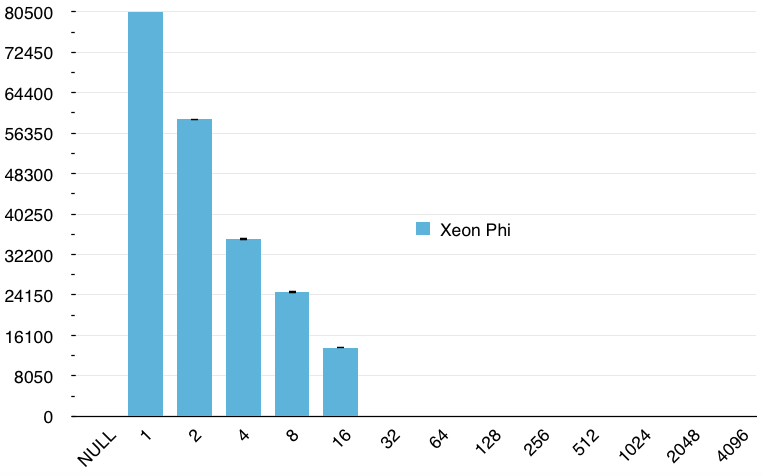
\includegraphics[width=0.49\textwidth]{figures/opt3_phi.png}
    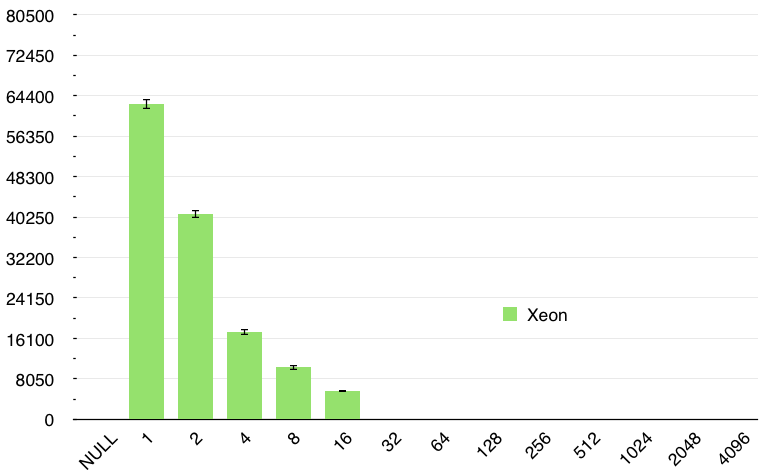
\includegraphics[width=0.49\textwidth]{figures/opt3_cpu.png}
    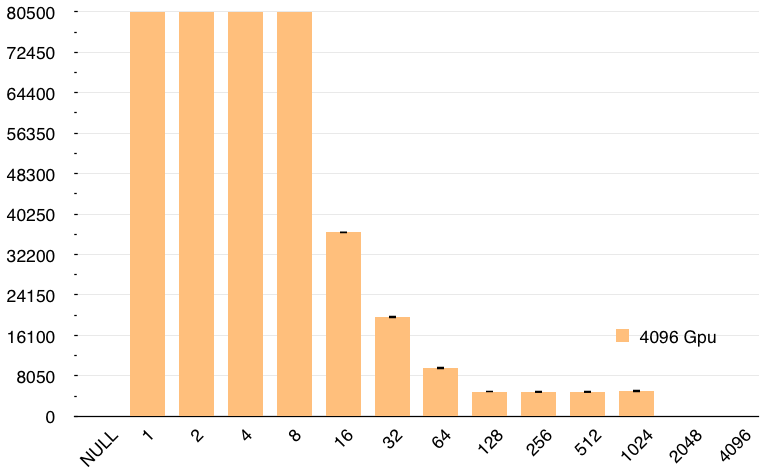
\includegraphics[width=0.49\textwidth]{figures/opt3_gpu.png}
    \caption{Rows and columns optimisation matrix multiplication in different architectures.}
    \label{RowsCols}
\end{figure}

\par{It seems to be a trade off here, between the the loop necesary to execute 
    the copy of elements of B to \emph{local memory}
    (expensive gathering operations with a very poor L1 hit ratio) and the 
    performance achieve in the loop where the kernel executes
    the computation(\emph{maybe vtune shot}).}

\par{In this case the best time is achived again by the GPU as we can see in 
    figure \ref{RowsColRes}, Also we can notice that the only 
    architectures that is able to take advantage of this optimisation is the 
    Xeon. The Xeon Phi even have a warning in its 
    documentation about not using \emph{local} memory explicitelly as in this 
    case, because of the cache system already is using 
    automatically this memory, and even warn about possible overhead time if 
    this memory is defined explicitely\cite{opencl_phi}.}

\begin{figure}[!h]
    \centering
    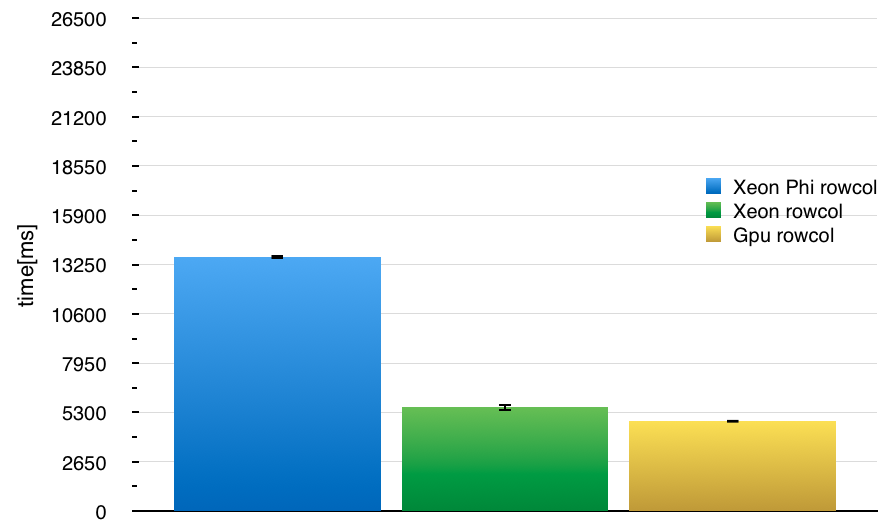
\includegraphics[width=0.49\textwidth]{figures/rowColRes.png}
    \caption{Rows and columns optimisation matrix multiplication best results in different devices.}
    \label{RowsColRes}
\end{figure}

